\documentclass[12pt,a4paper,oneside]{report}
\usepackage[utf8x]{inputenc}
\usepackage[brazil]{babel}
\usepackage[T1]{fontenc} 
\usepackage{ae}
\usepackage{indentfirst}

\usepackage{amsmath,amssymb,amsfonts,amstext}
\usepackage[hmarginratio=1:1,top=3cm,bottom=3cm,left=2cm,right=2cm,columnsep=20pt]{geometry}
\usepackage{graphicx}
%\usepackage{subfig}
\usepackage{float}
\usepackage{color}
\usepackage{xcolor}
\usepackage{listings}
\usepackage{subcaption}

\usepackage{multirow}
\usepackage{multicol}

\usepackage{algorithm}
\usepackage{algpseudocode}

\linespread{1.05} 
\usepackage{microtype} 
\usepackage{fancyhdr}
%\usepackage[sc]{mathpazo} 
%\usepackage[hang, small,labelfont=bf,up,textfont=it,up]{caption} 
\usepackage{booktabs}
\usepackage{paralist} 
\usepackage{abstract} 
\usepackage{titlesec} 
\usepackage[colorlinks=true, linkcolor=black, citecolor=black, urlcolor=black]{hyperref}
\usepackage{lmodern}
\usepackage[num]{abntex2cite}
\usepackage{makecell}


\renewcommand\theadalign{bc}
\renewcommand\theadfont{\bfseries}
\renewcommand\theadgape{\Gape[4pt]}
\renewcommand\cellgape{\Gape[4pt]}

\newcommand{\dpartial}[3][]{\dfrac{\partial^{#1} #2}{\partial #3^{#1}}}
\newcommand{\pbf}[1]{\noindent\textbf{#1}}
\newcommand{\pbfs}[1]{\noindent\textbf{#1}\\}
\newcommand{\degree}{^{\circ}}
\newcommand{\sen}{\text{sen}}
\newcommand{\senh}{\text{senh}}
\newcommand{\fig}[1]{Figura \ref{#1}}
\newcommand{\tab}[1]{Tabela \ref{#1}}
\newcommand{\eq}[1]{Equação (\ref{#1})}
\renewcommand{\abstractnamefont}{\normalfont\bfseries} 
\renewcommand{\abstracttextfont}{\normalfont\small\itshape} 
\newcommand{\jupyter}{Jupter Notebook\textsuperscript{\textregistered}\space}
\pagestyle{fancy}
\fancyhead{} 
\fancyfoot{}  
%\fancyhead[C]{Revista do Professor de Física $\bullet$ Brasília, vol. X, n. X $\bullet$ 20XX}
\fancyfoot[C]{\thepage}
%===================================================================================

%Definições de cor

\definecolor{mygreen}{rgb}{0,0.6,0}
\definecolor{mygray}{rgb}{0.5,0.5,0.5}
\definecolor{mymauve}{rgb}{0.58,0,0.82}

%Definições de citação

\citebrackets{[}{]}

%Definições de codigo
\renewcommand{\lstlistingname}{C\'odigo}
\renewcommand{\lstlistlistingname}{Lista de \lstlistingname s}
\lstset{ %
	backgroundcolor=\color{mygray!10},   % choose the background color; you must add \usepackage{color} or \usepackage{xcolor}
	basicstyle=\fontsize{9}{11}\selectfont\ttfamily,        % the size of the fonts that are used for the code
	breakatwhitespace=false,         % sets if automatic breaks should only happen at whitespace
	breaklines=true,                 % sets automatic line breaking
	captionpos=t,                    % sets the caption-position to bottom
	commentstyle=\color{mygreen},    % comment style
	%escapeinside={\%*}{*)},          % if you want to add LaTeX within your code
	extendedchars=true,              % lets you use non-ASCII characters; for 8-bits encodings only, does not work with UTF-8
	keepspaces=true,                 % keeps spaces in text, useful for keeping indentation of code (possibly needs columns=flexible)
	keywordstyle=\color{blue},       % keyword style
	language=python,                 	   % the language of the code
	numbers=left,                    % where to put the line-numbers; possible values are (none, left, right)
	numbersep=5pt,                   % how far the line-numbers are from the code
	numberstyle=\tiny\color{mygray}, % the style that is used for the line-numbers
	rulecolor=\color{black},         % if not set, the frame-color may be changed on line-breaks within not-black text (e.g. comments (green here))
	showspaces=false,                % show spaces everywhere adding particular underscores; it overrides 'showstringspaces'
	showstringspaces=false,          % underline spaces within strings only
	showtabs=false,                  % show tabs within strings adding particular underscores
	%  stepnumber=2,                    % the step between two line-numbers. If it's 1, each line will be numbered
	stringstyle=\color{mymauve},     % string literal style
	tabsize=4,	                   % sets default tabsize to 2 spaces
	title=\lstname,                   % show the filename of files included with \lstinputlisting; also try caption instead of title
	inputencoding=latin1,
	literate= %mapping letters
	{á}{{\'a}}1
	{à}{{\`a}}1
	{ã}{{\~a}}1
	{é}{{\'e}}1
	{ê}{{\^e}}1
	{í}{{\'i}}1
	{ó}{{\'o}}1
	{õ}{{\~o}}1
	{ú}{{\'u}}1
	{ü}{{\"u}}1
	{ç}{{\c{c}}}1
}


%===================================================================================

\title{\vspace{-5mm}\fontsize{18pt}{10pt}
	% COLOQUE AQUI O TÍTULO DO SEU TRABALHO
	\vspace*{-100pt}
	\begin{center}
		\begin{minipage}{0.20\textwidth}
			\centering 
\includegraphics[width=1.2\textwidth]{img/ufrj-logo.png}
		\end{minipage}
	\end{center}
	\normalfont\textsc{Universidade Federal do 
		Rio de Janeiro \\ 
		Programa de Pós-graduação em Engenharia Mecânica - COPPE}\\
	\vspace*{100pt}
	
	\bf{Análise do Ruído em Aerofólios com Redes Neurais}
	\vspace*{30pt}
}
\author{
	\large 
	% COLOQUE AQUI O NOME DO PRIMEIRO AUTOR
	\textsc{Bruno da Silva Machado}
}
\date{\today}

\begin{document}
	
	\maketitle
	
	\pagenumbering{roman}
	\setcounter{page}{1}
	
	\begin{abstract}
	Neste trabalho, foi desenvolvida uma rede neural do tipo Multi-Layer Perceptron (MLP) com o objetivo de modelar a pressão sonora gerada por aerofólios, utilizando um conjunto de dados experimental da NASA. A abordagem envolveu a análise exploratória dos dados, com destaque para a identificação de outliers, correlação entre variáveis e normalização com escore Z. Em seguida, o modelo MLP foi treinado com TensorFlow, utilizando uma camada oculta de 10 neurônios, função de ativação sigmoide e otimização com decaimento exponencial da taxa de aprendizado. Avaliou-se o desempenho por meio de métricas como MSE, MAE, RAE e $R^2$, além de gráficos de resíduos e comparação com regressão linear. Também foram realizados experimentos para analisar a influência da complexidade da rede e a capacidade de extrapolação. 
	Os resultados indicaram que a MLP supera modelos lineares tradicionais em capacidade preditiva, e embora a extrapolação represente um desafio para redes neurais, o modelo demonstrou estabilidade e coerência nas predições mesmo fora da faixa de treino.
	%Os resultados indicaram que a MLP supera modelos lineares tradicionais, porém, sua capacidade de extrapolação é limitada, reforçando a importância da cobertura adequada do espaço de entrada.
		
		
	\end{abstract}
	
		%%%%%%%%%%%%%%%%%%%%%%%%%%%%%%%%%%%%%%%%%%%%%%%%%%%%%%%%
	%                   Lista de Figuras                   %
	%%%%%%%%%%%%%%%%%%%%%%%%%%%%%%%%%%%%%%%%%%%%%%%%%%%%%%%%
	%
	\listoffigures
	%
	\addcontentsline{toc}{chapter}{Lista de Figuras}
	
	
	%%%%%%%%%%%%%%%%%%%%%%%%%%%%%%%%%%%%%%%%%%%%%%%%%%%%%%%%
	%                   Lista de Tabelas                   %
	%%%%%%%%%%%%%%%%%%%%%%%%%%%%%%%%%%%%%%%%%%%%%%%%%%%%%%%%
	%
	\listoftables
	%
	\addcontentsline{toc}{chapter}{Lista de Tabelas}
	
	%%%%%%%%%%%%%%%%%%%%%%%%%%%%%%%%%%%%%%%%%%%%%%%%%%%%%%%%
	%                   Lista de Código                    %
	%%%%%%%%%%%%%%%%%%%%%%%%%%%%%%%%%%%%%%%%%%%%%%%%%%%%%%%%
	%
	\lstlistoflistings
	%
	\addcontentsline{toc}{chapter}{Lista de Códigos}
	
	%%%%%%%%%%%%%%%%%%%%%%%%%%%%%%%%%%%%%%%%%%%%%%%%%%%%%%%%
	%                       Sumário                        %
	%%%%%%%%%%%%%%%%%%%%%%%%%%%%%%%%%%%%%%%%%%%%%%%%%%%%%%%%
	%
	\addcontentsline{toc}{chapter}{Sumário}
	
	\tableofcontents
	
	%%%%%%%%%%%%%%%%%%%%%%%%%%%%%%%%%%%%%%%%%%%%%%%%%%%%%%
	%                Numeracao em arabico                %
	%%%%%%%%%%%%%%%%%%%%%%%%%%%%%%%%%%%%%%%%%%%%%%%%%%%%%%
	%
	\clearpage
	%
	\pagenumbering{arabic}
	
	\chapter{Multi-Layer Perceptron}
	\label{sec:introducao}
	
	\section{O que é o Multi-Layer Perceptron}
	
%	O Perceptron Multicamadas (MLP, do inglês \textit{Multi-Layer Perceptron}) é uma arquitetura de rede neural feedforward composta por uma camada de entrada, uma ou mais camadas ocultas e uma camada de saída. As MLPs s\~ao amplamente utilizadas em tarefas de regress\~ao e classifica\c{c}\~ao, principalmente por sua capacidade de modelar rela\c{c}\~oes n\~ao lineares complexas.
%	
%	A dedu\c{c}\~ao do MLP parte do perceptron simples, em que cada neurônio realiza uma soma ponderada das entradas seguida de uma fun\c{c}\~ao de ativa\c{c}\~ao. Com a introdu\c{c}\~ao de camadas ocultas, o modelo pode capturar padr\~oes mais complexos, aumentando sua capacidade expressiva.
%	
%	\begin{center}
%		\includegraphics[width=0.7\textwidth]{mlp\_diagrama.png} % Inserir diagrama posteriormente
%	\end{center}
%	
%	No contexto da mecânica dos fluidos, o ruído gerado em aerofólios é resultado de fenômenos aerodinâmicos como o escoamento turbulento e a separa\c{c}\~ao da camada limite. Este trabalho analisa um conjunto de dados experimentais da NASA com o objetivo de prever o nível de press\~ao sonora a partir de variáveis como: frequência, ângulo de ataque, comprimento da corda, velocidade de fluxo livre e espessura de suc\c{c}\~ao.
	
	O Multi-Layer Perceptron (MLP) é uma das principais arquiteturas de redes neurais adaptativas, composta por várias camadas de neurônios, cada uma com pesos ajustáveis\cite{tracker:2024}\cite{culturamix:2009}. %O MLP tem o propósito de representar um mapeamento entrada-saída qualquer, aproximado-os
	Os MLPs s\~ao amplamente utilizados em tarefas de regress\~ao e classifica\c{c}\~ao, principalmente por sua capacidade de modelar rela\c{c}\~oes n\~ao lineares complexas.
	
	Um Multi-Layer Perceptron é composto por várias camadas chamadas de perceptrons, unidade básica de processamento. Um perceptron recebe um conjunto de entradas, realiza uma combinação linear dessas entradas com pesos associados e aplica uma função de ativação para gerar uma saída. Em um MLP cada perceptron é conectado à camada seguinte por meio de pesos ajustáveis\cite{tracker:2024}.  
	
	Na \fig{fig:camadas} mostramos a arquitetura de uma rede neural Multi-Layer Perceptron. A primeira camada (em azul) é a camada de entrada, que recebe os dados brutos. As camadas intermediárias (em vermelho) são chamadas de ocultas, pois não é possível prever a saída desejada nessas camadas intermediárias e a última camada (em amarelo) é a saída, onde os erros de aproximação são calculados e a resposta final do modelo é produzida\cite{moreira:2018}.
\begin{figure}[th!]
	\centering
	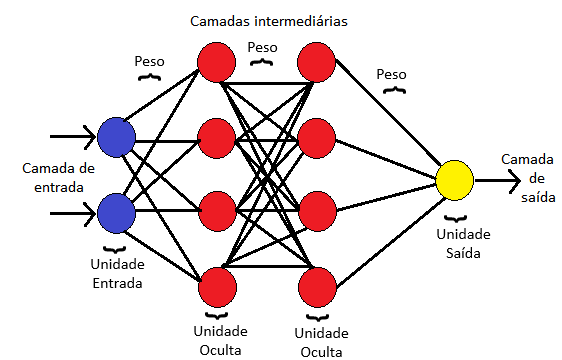
\includegraphics[width=0.6\linewidth]{img/camadas}
	\caption[Diagrama Multi-Layer Perceptron]{Diagrama de uma rede neural Multi-Layer Perceptron}
	\label{fig:camadas}
\end{figure}

	\section{Função de Ativação}
	Uma função de ativação é aplicada em cada perceptron para introduzir não linearidades no modelo. Isso permite que o MLP aprenda relações complexas nos dados. Alguns exemplos de funções de ativação comumente usadas são a função sigmoide, a função ReLU e a função tangente hiperbólica. Neste trabalho será utilizado a função sigmoide devido a sua simplicidade e versalidade.
	
	\subsection{Função Sigmoide}
	
	A função sigmoide ou logística é uma função de ativação dada por:
	\begin{equation}
		\sigma(x) = \frac{1}{1 + e^{-x}}
	\end{equation}
	
	Ela tem as seguintes propriedades:
	\begin{itemize}
		\item A função é infinitesimalmente suave e monótona.
		\item O intervalo da função é entre $(0,1)$, ou seja, é uma função limitada. Esta função é utilizada na representação probabilística.
		\item Como a derivada decai rapidamente para zero a partir de $\epsilon = 0$, essa função de ativação pode levar a convergência lenta da rede durante o treinamento\cite{ray2023deeplearningcomputationalphysics}.
	\end{itemize}

\begin{figure}[th!]
	\centering
	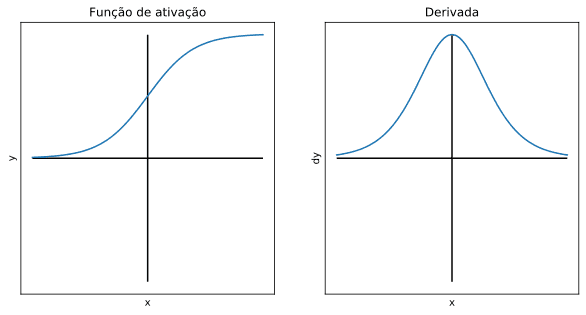
\includegraphics[width=0.6\linewidth]{img/sigmoide}
	\caption[Função sigmoide e sua derivada.]{Função sigmoide e sua derivada.}
	\label{fig:sigmoide}
\end{figure}

Na \fig{fig:sigmoide} a função Sigmoide mapeia todos os valores reais, $x$, para um intervalo limitado entre $(0,1)$ de forma continua e suave. Além disso, a sua derivada é a função gaussiana que mapeia todos os pontos em uma distribuição e pode ser interpretado com uma distribuição de probabilidade, útil em problemas de classificação. 

Entretanto, sua característica não-linear aumenta o custo computacional. Além disso, como observado na \fig{fig:sigmoide}, a função sigmoide não é centrada em zero. Não só isso, ela apresenta platôs para valores de $x$ muito altos ou muito baixos, o que faz com que a derivada nessas regiões se aproxime de zero. A soma dessas características não faz da função sigmoide uma boa opção para ativação das camadas escondidas.
	
\section{Regularização L2}

A regularização é um conjunto de métodos para reduzir o overfitting em modelos de aprendizado de máquina. Normalmente, a regularização troca uma leve redução na precisão do treinamento por um aumento na capacidade de generalização\cite{murel:2023}.

A regularização L2 é uma técnica de regularização que penaliza coeficientes de alto valor ao introduzir um termo de penalização na função de custo\cite{murel:2023}. 

A fun\c{c}\~ao de custo escolhida foi o Erro Quadrático Médio (MSE), pois penaliza erros maiores de forma mais significativa:
\begin{equation}
	\label{eq:mse}
	MSE = \frac{1}{n}\sum_{i=1}^n (y_i - \hat{y}_i)^2
\end{equation}

Para evitar overfitting, incluímos o termo de regulariza\c{c}\~ao L2:
\begin{equation}
	J(\theta) = MSE + \lambda \sum \theta^2
\end{equation}

Portanto a função de custo é a soma do MSE com a regularização L2. A vantagem de construir a função custo dessa forma é corrigir o overfitting e a desvantagem é o risco de subajuste caso o modelo receba viés excessivo por meio da regularização.
	
	\section{Retropropagação de Erro (Backpropagation)}
	
	Comumente é utilizado o algoritmo de retropropagação do erro para treinar a rede neural MLP\cite{moreira:2018}.
	
	A ideia do algoritmo de retropropagação se baseia no cálculo do erro obtido na camada de saída da rede neural. Deve-se ajustar os valores dos pesos e limites conforme o erro e retro-propagado. O procedimento que algoritmo faz é calcular o erro entre o que foi obtido pela rede e o valor esperado, então ajustar os valores de todos os pesos, começando pelos pesos da camada de saída e retrocedendo até a entrada, sempre tentando minimizar este erro.
	
	O algoritmo de retropropagação segue os seguintes etapas:
	
	\begin{itemize}
		\item Inicializa os pesos da rede com uma distribuição normal e uniforme de valores aleatórios;
		
		\item Fornece dados de entrada a rede e calcula o valor da função de erro obtida, ao comparar com o valor de saída esperado;
		
		\item Busca-se minimizar o valor da função de erro calculando os valores dos gradientes para cada peso da rede, uma vez que o gradiente fornece a direção de maior crescimento, bastando escolher o sentido contrário do gradiente;
		
		\item Com o vetor gradiente calculado, ajusta-se cada peso de maneira iterativa. Deve-se recalcular os gradientes a cada passo de iteração, até o erro atingir algum limiar, ou alcançar o número máximo de iterações.
	\end{itemize}
	
	\subsection{Implementação do algoritmo de Retropropagação de Erro (Backpropagation)}
	\label{sec:impl_mlp}
	
	Nessa seção, adaptamos a demonstração do algoritmo de backpropagation \cite{leite:2018} para a arquitetura específica da rede utilizada neste projeto: uma rede neural com 5 neurônios de entrada, 10 neurônios na camada intermediária (camada oculta) e 1 neurônio de saída. A função de ativação utilizada é a sigmoide, e a função de erro é o erro quadrático médio (MSE).
	
	A fórmula geral de atualização dos pesos em uma iteração do algoritmo é:
	
	\begin{equation}\label{eq:wdate}
		w \leftarrow w - \eta \frac{\partial E}{\partial w},
	\end{equation}
	
	ou seja, o valor do peso $w$ na iteração atual será o valor anterior, corrigido de valor proporcional ao gradiente. O sinal negativo significa que estamos indo na direção contrária à do gradiente. O parâmetro $\eta$ representa a taxa de aprendizado da rede neural, controlando a largura do passo na correção do peso. 
	
	Na equação (\ref{eq:wdate}), o principal conceito é o cálculo das derivadas parciais da função de erro em relação ao vetor de pesos $w$. A figura \ref{fig:mlp_backprop_diagram} temos uma rede perceptron multicamada com um camada intermediária. Uma junção entre um neurônio $j$ e um neurônio $i$ da camada seguinte possui peso $w_{ij}$. Os números sobrescritos, entre parênteses, indicam o número da camada a qual a variável pertence.
	
	\begin{figure}[h]
		\centering
		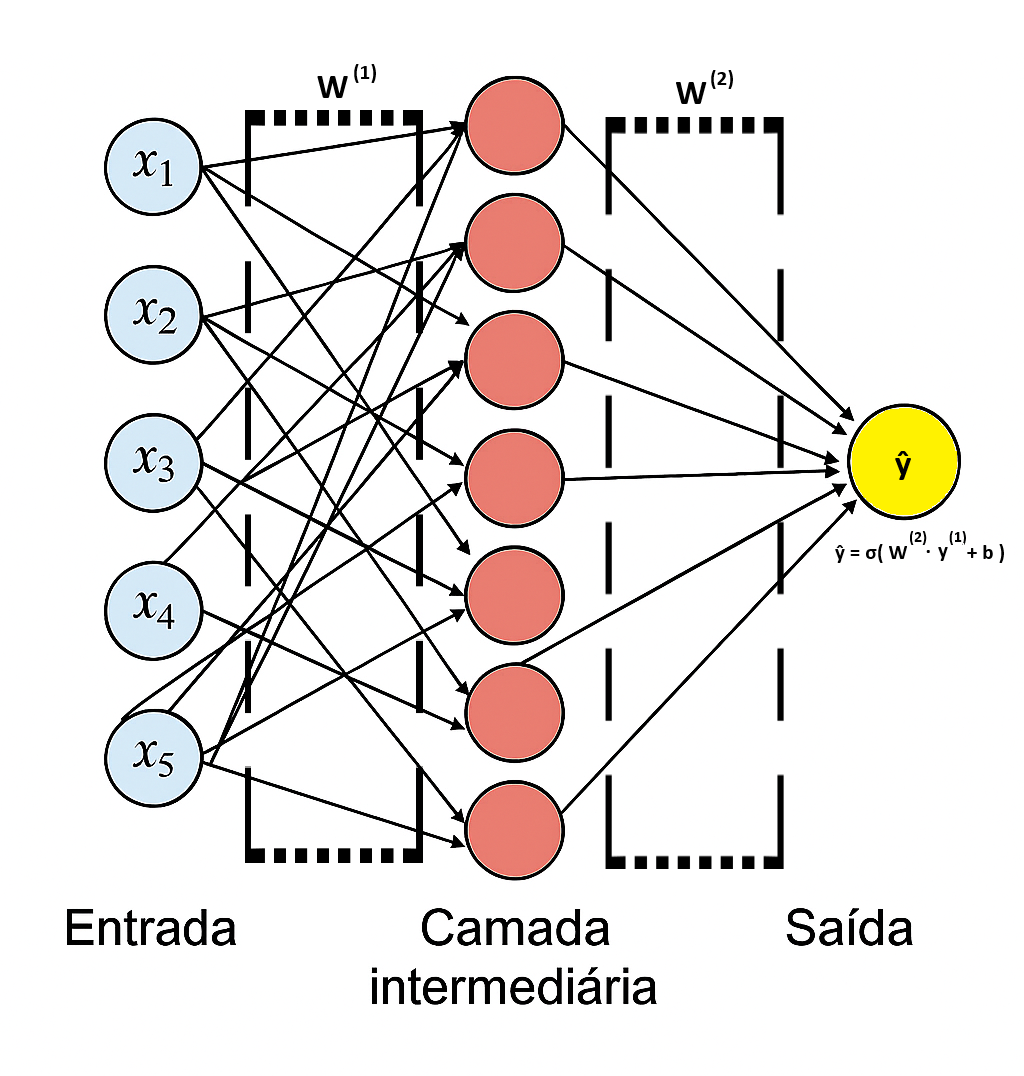
\includegraphics[width=0.6\linewidth]{img/mlp_backprop_diagram}
		\caption[Implementação do Multi-Layer Perceptron]{ Implementação da rede neural MLP para a explicação da retropropagação}
		\label{fig:mlp_backprop_diagram}
	\end{figure}

Na \fig{fig:mlp_backprop_diagram} temos em cada circulo azul a representação das entadas do conjunto $\mathbf{x}$, os círculos vermelhos representam as camadas intermediárias e em amarelo a saída $\hat{y} = \sigma(\mathbf{W}^{(2)} \cdot y^{(1)} + \mathbf{b}^{(2)})$
	
	Considerando a arquitetura da rede: uma camada de entrada com 5 variáveis $\mathbf{x} = (x_1, x_2, x_3, x_4, x_5)$, conectada a uma camada oculta com 10 neurônios. Os potenciais de ativação da camada oculta são:
	
	\begin{equation}
		z_j^{(1)} = \sum_{i=1}^{5} w_{i,j}^{(1)} x_i + b_j^{(1)}, \quad j = 1, ..., 10
	\end{equation}
	
	E suas saídas são:
	
	\begin{equation}
		y_j^{(1)} = \sigma(z_j^{(1)})
	\end{equation}
	
	A camada de saída é composta por um único neurônio, com entrada total:
	
	\begin{equation}
		z^{(2)} = \sum_{j=1}^{10} w_j^{(2)} y_j^{(1)} + b^{(2)}
	\end{equation}
	
	E saída final:
	
	\begin{equation}
		\hat{y} = \sigma(z^{(2)})
	\end{equation}
	
	O erro quadrático médio é definido como $\sum_{i}^{N} (y_i - \hat{y}_i)^2/\text{N}$. Entretanto temos apenas duas saídas então podemos simplificar o erro quadrático médio para uma amostra:
	
	\begin{equation}
		E = \frac{1}{2}(y - \hat{y})^2
	\end{equation}
	
	Aplicando a regra da cadeia, calculamos a derivada do erro em relação à saída predita:
	
	\begin{equation}
		\frac{\partial E}{\partial \hat{y}} = -(y - \hat{y})
	\end{equation}
	
	Como $\hat{y} = \sigma(z^{(2)})$, temos:
	
	\begin{equation}
		\frac{\partial E}{\partial z^{(2)}} = \frac{\partial E}{\partial \hat{y}} \cdot \sigma'(z^{(2)}) = -(y - \hat{y}) \cdot \hat{y}(1 - \hat{y})
	\end{equation}
	
	Chamamos esse termo de $\delta^{(2)}$:
	
	\begin{equation}
		\delta^{(2)} = -(y - \hat{y}) \cdot \hat{y}(1 - \hat{y})
	\end{equation}
	
	Calculamos as derivadas parciais do erro em relação aos pesos e viés da camada de saída:
	
	\begin{equation}
		\frac{\partial E}{\partial w_j^{(2)}} = \delta^{(2)} y_j^{(1)}, \quad \frac{\partial E}{\partial b^{(2)}} = \delta^{(2)}
	\end{equation}
	
	O que gera as seguintes atualizações:
	
	\begin{equation}
		w_j^{(2)} \leftarrow w_j^{(2)} - \eta \delta^{(2)} y_j^{(1)}, \quad b^{(2)} \leftarrow b^{(2)} - \eta \delta^{(2)}
	\end{equation}
	
	Agora, propagamos o erro para a camada oculta. Para cada neurônio oculto $j$, temos:
	
	\begin{equation}
		\delta_j^{(1)} = \delta^{(2)} w_j^{(2)} \cdot \sigma'(z_j^{(1)}) = \delta^{(2)} w_j^{(2)} y_j^{(1)} (1 - y_j^{(1)})
	\end{equation}
	
	Derivadas parciais do erro em relação aos pesos e viés da camada oculta:
	
	\begin{equation}
		\frac{\partial E}{\partial w_{i,j}^{(1)}} = \delta_j^{(1)} x_i, \quad \frac{\partial E}{\partial b_j^{(1)}} = \delta_j^{(1)}
	\end{equation}
	
	Atualizamos os pesos da camada oculta:
	
	\begin{equation}
		w_{i,j}^{(1)} \leftarrow w_{i,j}^{(1)} - \eta \delta_j^{(1)} x_i, \quad b_j^{(1)} \leftarrow b_j^{(1)} - \eta \delta_j^{(1)}
	\end{equation}
	
	Com essas equações, implementamos de forma sistemática o algoritmo de retropropagação adaptado à estrutura da rede neural deste projeto, com propagação do erro e atualização dos pesos desde a camada de saída até as entradas.

\chapter{Introdução ao TensorFlow}

Na seção \ref{sec:impl_mlp} implementamos um algoritmo para a retropropagação do erro. Apesar disso, nesse trabalho foi utilizado a biblioteca TensorFlow para implementar e treinar a rede neural MLP.
%	- tensorflow
%	- MLP com tensorflow
%	- taxa de aprendizado decaimento exponencial.

\section{O que é o TensorFlow}

O TensorFlow é uma biblioteca de código aberto desenvolvida pela equipe do Google Brain, projetada para facilitar o desenvolvimento e a execução de algoritmos de aprendizado de máquina, especialmente redes neurais profundas. Ele permite a construção de modelos computacionais usando grafos de fluxo de dados, onde os nós representam operações matemáticas e as arestas representam tensores que são estruturas de dados multidimensionais \cite{wikipedia:2022}.

A principal vantagem do TensorFlow está na flexibilidade. Ele pode ser utilizado em ambientes de produção com alto desempenho (via GPU e TPU), bem como em dispositivos móveis e navegadores, graças ao TensorFlow Lite e TensorFlow.js \cite{didatica:2024}. Além disso, é amplamente utilizado tanto na indústria quanto na academia para tarefas de classificação, regressão, processamento de linguagem natural, visão computacional, entre outras.

\section{Multi-Layer Perceptron com TensorFlow}
\label{sec:mpl_tf}
Um \textit{Multi-Layer Perceptron} (MLP) é uma rede neural \textit{feedforward} composta por camadas densamente conectadas (ou densas), normalmente contendo uma camada de entrada, uma ou mais camadas ocultas e uma camada de saída. Cada camada é composta por neurônios que aplicam uma transformação linear seguida de uma função de ativação não linear, como ReLU ou Sigmoid.

No TensorFlow, um MLP pode ser implementado usando a API \texttt{tf.keras.Sequential}, que permite empilhar camadas de maneira simples e direta. Por exemplo:
\begin{lstlisting}[caption={implementação MLP no tensorflow}, label={lst:impl_tf}]
	import tensorflow as tf
	from tensorflow.keras.models import Sequential
	from tensorflow.keras.layers import Dense
	
	model = Sequential([
	Dense(10, activation='sigmoid', input_shape=(X.shape[1],)),
	Dense(1, activation='linear')  # saída contínua
	])
\end{lstlisting}

No código \ref{lst:impl_tf} o modelo é criado pela classe \texttt{Sequential()} que define um conjunto de camadas lineares. A camada \texttt{Dense(10, activation=`sigmoid')} possui 10 neurônios e utiliza a função de ativação sigmoide. O parâmetro \texttt{input\_shape} define a dimensão da entrada. A camada de saída tem um único neurônio de saída, com ativação \texttt{linear}, adequada para regressão. 

Após a definição da arquitetura, o modelo é compilado e treinado:

\begin{lstlisting}[caption={Compilar e Treinar o Modelo}, label={lst:compl_tf}]
	model.compile(optimizer='adam',loss='mse',metrics=['mae'])
	
	model.fit(x_train, y_train, epochs=200, batch_size=32)
\end{lstlisting}

No método \texttt{modelo.compile()} o otimizador \texttt{Adam} é utilizado por ser eficiente e adaptativo. A função de perda \texttt{mse} é o erro quadrático médio definido na equação \ref{eq:mse}. O treinamento é realizado por 200 épocas com mini-lotes de 32 amostras.

O TensorFlow gerencia automaticamente os gradientes e a retropropagação (\textit{backpropagation}), simplificando o treinamento do modelo \cite{geeksforgeeks:2025, leite:2018aug}.

\section{Taxa de Aprendizado com Decaimento Exponencial}

A taxa de aprendizado é um dos hiperparâmetros mais importantes no treinamento de redes neurais. Ela define o tamanho dos passos que o otimizador dá em direção ao mínimo da função de perda. Uma taxa muito alta pode fazer o modelo divergir, enquanto uma taxa muito baixa pode torná-lo extremamente lento para convergir.

Para lidar com essa sensibilidade, o TensorFlow oferece mecanismos para alterar dinamicamente a taxa de aprendizado durante o treinamento. Um método comum é o \textit{decaimento exponencial} (\textit{exponential decay}), onde a taxa de aprendizado diminui exponencialmente ao longo do tempo. Isso permite passos maiores no início do treinamento e passos mais precisos na fase final de ajuste fino.

No TensorFlow, isso pode ser implementado com:
\begin{lstlisting}[caption={Decaimento exponencial}, label={lst:exp_dacay}]
	lr_schedule = tf.keras.optimizers.schedules.ExponentialDecay(
	initial_learning_rate=0.01,
	decay_steps=100000,
	decay_rate=0.96,
	staircase=True)
	
	optimizer = tf.keras.optimizers.Adam(learning_rate=lr_schedule)
\end{lstlisting}

Onde 
\begin{itemize}
	\item \texttt{initial\_learning\_rate=0.01} define a taxa inicial de aprendizado.
	\item \texttt{decay\_steps=100000} indica que a taxa será atualizada a cada 100.000 passos de treinamento.
	\item \texttt{decay\_rate=0.96} significa que a taxa de aprendizado será multiplicada por 0.96 a cada \texttt{decay\_steps}.
	\item \texttt{staircase=True} faz com que o decaimento ocorra em degraus (em vez de contínuo), criando uma curva em escada.
	\item O otimizador Adam é então criado utilizando esse agendador de taxa de aprendizado.
\end{itemize}

Esse tipo de abordagem ajuda a obter um treinamento mais estável e eficaz, especialmente em redes neurais profundas \cite{databricks:2024}.
	
	\chapter{Resultados}
	Neste projeto, foi construído uma rede neural para analisar e modelar um conjunto de dados experimentais produzido pelo NASA no final dos anos 80. Esses dados foram produzidos em um túnel de vento e visavam compreender a produção de ruído no entorno de uma asa. Na mecânica dos fluídos o problema do ruído em aerofólios está relacionado à geração de ruído por meio de fenômenos aerodinâmicos, como o escoamento turbulento e a separação da camada limite.
	
	Essa seção foi dividida em duas parte: A primeira parte foram realizadas análises  na descrição estatística dos dados, nos gráficos de dispersão e histogramas, na correlação dos dados e por fim na localização de outliers e normalização dos dados. A segunda parte foi realizado o treinamento e validação da rede neural MLP, além de avaliar três cenários possíveis que são a variação do número de neurônios, a comparação da rede neural com outros modelos e a extrapolação dos dados.
	
	\section{Análise dos Dados}
	
	O conjunto de dados da NASA compreende aerofólios NACA 0012 \cite{airfoil_self-noise_291} de tamanhos diferentes em várias velocidades de túnel de vento e ângulos de ataque. A envergadura do aerofólio e a posição do observador foram as mesmas em todos os experimentos. Não há valores ausentes nesse conjunto de dados.
	
	\pbfs{Informações sobre as variáveis.}
	
	Esse problema tem as seguintes entradas:
	\begin{itemize}
		\item Frequência, em Hertzs.
		\item Ângulo de ataque, em graus.
		\item Comprimento da corda, em metros.
		\item Velocidade de fluxo livre, em metros por segundo.
		\item Espessura do deslocamento do lado da sucção, nos medidores. 
	\end{itemize}
	A única saída é: Nível de pressão sonora escalonado, em decibéis.
	
	Na \tab{tab:est_naca_0012} temos a análise descritiva do conjunto de dados nela podemos verificar algumas informações uteis dos dados antes de realizar o treinamento da rede neural.
	\begin{table}[h!]
		\centering
		\caption{Estatísticas descritivas das variáveis}
		\label{tab:est_naca_0012}
		\begin{tabular}{lcccccc}
			\toprule
			& \thead{Frequência} & \thead{Angulo de\\ Ataque} & \thead{Comprimento\\ da Corda} & \thead{Velocidade\\ do Fluxo }& \thead{Espessura\\ Suc\c{c}\~ao} & \thead{Press\~ao\\ Sonora} \\
			\midrule
			média& 2886,380&	6,782&	0,136&	50,860&	0,011&	124,835\\
			std&	3152,573&	5,918&	0,094&	15,572&	0,013150&	6,899\\
			min&	200,000&	0,000&	0,0254&	31,700&	0,000401&	103,380\\
			25\%&	800,000&	2,000&	0,051&	39,600&	0,002535&	120,191\\
			50\%&	1600,000&	5,400&	0,102&	39,600&	0,004957&	125,721\\
			75\%&	4000,000&	9,900&	0,229&	71,300&	0,0156&	129,995\\
			máx&	20000,000&	22,200&	0,305&	71,300&	0,0584&	140,987\\
			\bottomrule
		\end{tabular}
	\end{table}

Na \fig{fig:t1boxplot} complementamos a analise com gráficos de boxplots. Um boxplot é um diagrama de caixa que mostra o resumo das propriedades de um conjunto de valores numéricos como mínimo, primeiro quartil, mediana, terceiro quartil e máximo.
\begin{figure}[th]
	\centering
	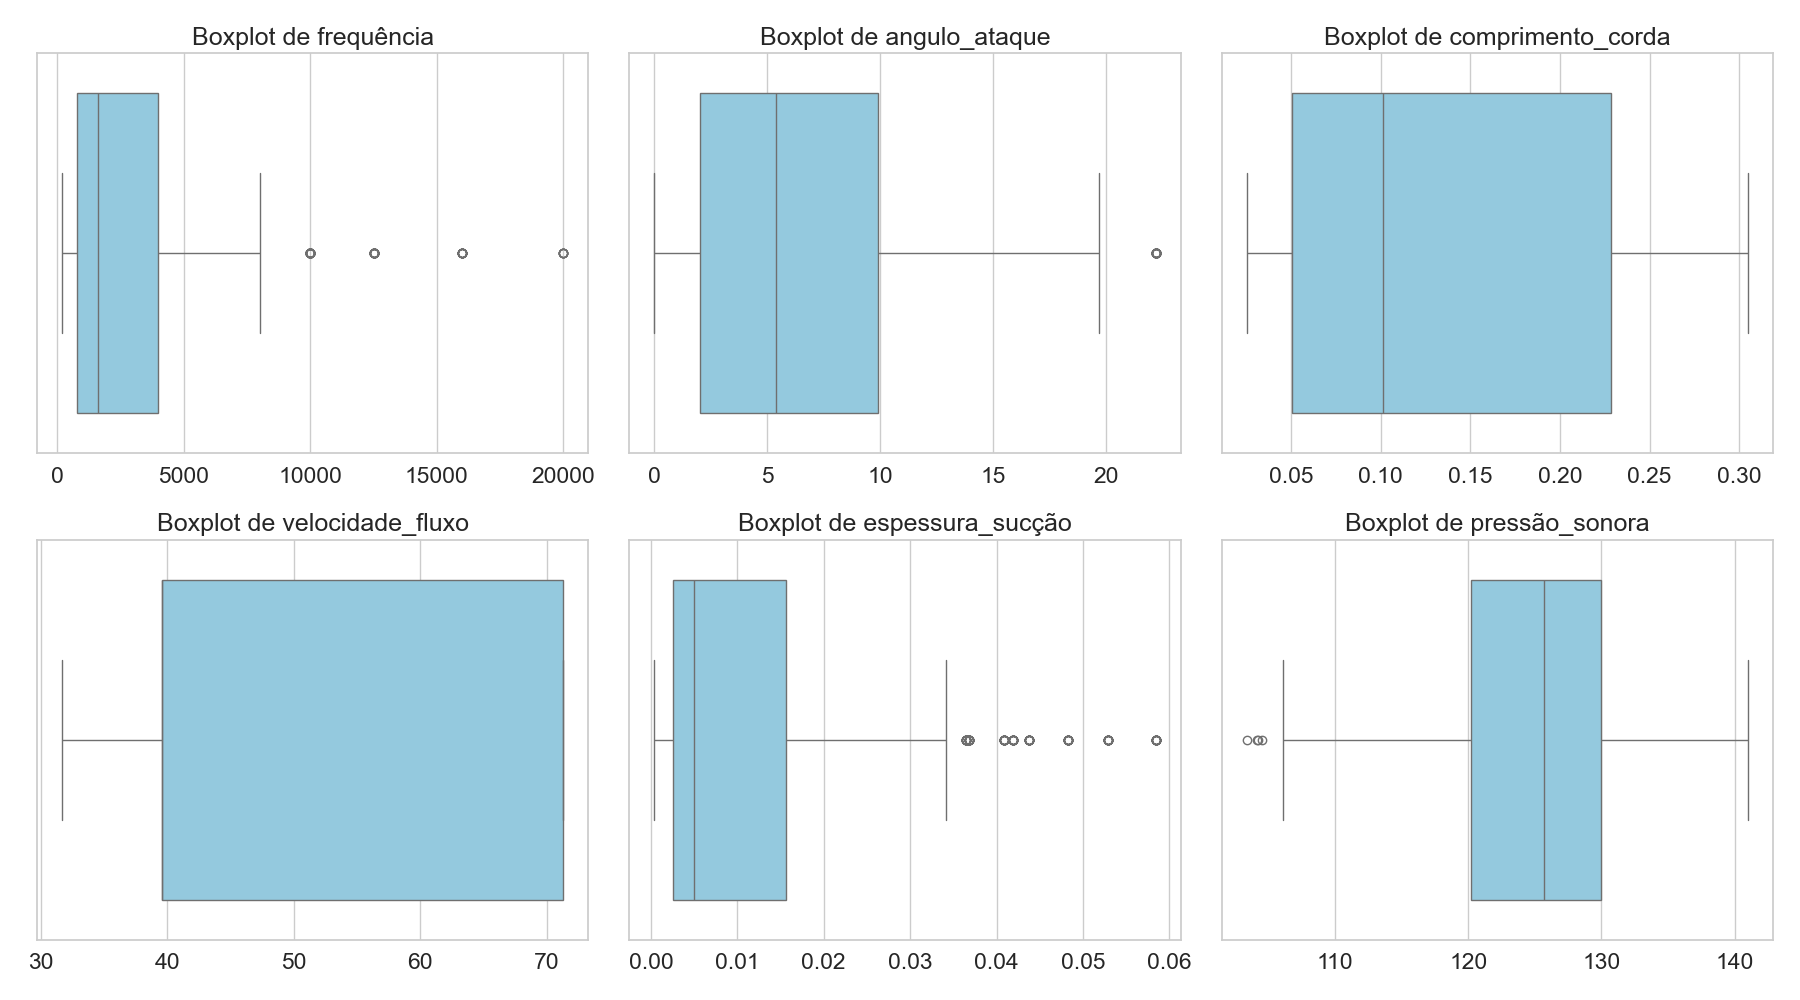
\includegraphics[width=0.8\paperwidth]{img/t1_boxplot}
	\caption{Boxplot do conjunto de dados}
	\label{fig:t1boxplot}
\end{figure}

Analisando os valores da coluna \texttt{Frequência} temos uma média de $2886,38 \text{ Hz}$ e um desvio padrão (\texttt{std}) de aproximadamente $3152,57 \text{ Hz}$ isso indica uma alta dispersão e um desvio muito elevado, além disso o intervalo é de  $200,00 \text{ Hz}$ a $20.000,00 \text{ Hz}$, ou seja, há uma grande amplitude. Na \fig{fig:t1boxplot}a podemos verificar que há vários outliers no extremo superior.

Na coluna \texttt{Ângulo de ataque} temos uma média de $6,782\degree$ e um desvio padrão de $5,918\degree$ o que é uma dispersão moderada. A mediana de $5,4\degree$ é um pouco menor que a média, indicando possível leve assimetria à direita.  Na \fig{fig:t1boxplot}b observamos uma distribuição compacta, sem outliers visíveis e dados bem comportados.

Na coluna \texttt{Comprimento da corda} a mediana de $0,102\text{ m}$ é menor que a média ($0,136 \text{ m}$), sugerindo presença de valores maiores extremos. Na \fig{fig:t1boxplot}c não consta outliers relevantes e variação pequena.

Na coluna \texttt{Velocidade do fluxo} temos um comportamento curioso: A velocidade mínima é de $31,7\text{ m/s}$, mas o valor de 75\% é igual ao máximo $(71,3\text{ m/s})$, indicando uma possível concentração no valor máximo. Na \fig{fig:t1boxplot}d constamos uma distribuição bem centrada, sem outliers aparentes.

Na coluna \texttt{Espessura de sucção} a média é muito maior que a mediana $(0,004957\text{ m})$, o que indica uma forte assimetria à direita, ou seja, valores extremos altos. Alguns outliers são visíveis no lado superior.

Na coluna \texttt{Pressão sonora} a mediana $(125,721\text{ dB})$ é um pouco maior que a média $(124,835\text{ dB})$, sugerindo uma leve assimetria à esquerda. Alguns poucos outliers inferiores, mas a maioria dos dados está bem distribuída.
	
	%Foram gerados boxplots para cada variável, gráficos de dispers\~ao, histogramas com curvas de tendência e gráficos logarítmicos para as variáveis mais influentes. A rela\c{c}\~ao entre entradas e saída também foi analisada com suaviza\c{c}\~ao LOWESS.
	
\subsection{Gráficos de dispersão com LOWESS}

Utilizamos gráficos de dispersão para mostra os valores de duas variáveis, permitindo visualizar padrões, tendências e dispersões. No contexto de regressão, queremos ver como cada variável de entrada se relaciona com a variável de saída (pressão).

Para aprofundar a análise foi utilizado o LOWESS (ou LOESS) que significa \textit{Locally Weighted Scatterplot Smoothing}. É um método não paramétrico que ajusta uma curva suave sobre os dados no gráfico de dispersão ao realizar regressões locais ponderadas, revelando relações não lineares entre as variáveis. o LOWESS não assume uma forma específica da relação (linear, polinomial, etc.) e a curva é ajustada localmente em torno de cada ponto. Assim devemos interpretar os gráficos da seguinte forma:
\begin{itemize}
	\item Se a curva não for reta, isso indica uma relação não linear.
	\item Uma curva descendente indica que, à medida que a variável aumenta, a pressão sonora tende a diminuir (e vice-versa).
	\item Ondulações ou curvaturas mais complexas sugerem relações mais complicadas, que redes neurais conseguem modelar melhor do que modelos lineares.
\end{itemize}
Na \fig{fig:t1disperssaolowessfrequencia} a curva mostra uma clara tendência decrescente. Isso confirma a correlação negativa moderada: conforme a frequência aumenta, a pressão sonora tende a diminuir. Relação não linear suave, com declínio mais acentuado em frequências mais baixas.

Na \fig{fig:t1disperssaolowessanguloataque} a curva tem uma leve queda, mas quase plana. Confirma que há pouca influência direta, talvez com pequenas oscilações não lineares. Pode indicar que esta variável tem influência condicional em interação com outras variáveis.
\begin{figure}[H]
	\centering
	\includegraphics[width=0.5\linewidth]{img/t1_disperssao_lowess_frequência}
	\caption{Frequência (Hz) vs Pressão Sonora (dB)}
	\label{fig:t1disperssaolowessfrequencia}
\end{figure}

Na \fig{fig:t1disperssaolowesscomprimentocorda} a relação é ligeiramente não linear, com uma tendência decrescente. Sugere que aerofólios com corda maior tendem a produzir um pouco menos de ruído. A não linearidade é suave, o que pode ser modelado por redes neurais.
\begin{figure}[!h]
	\begin{subfigure}{0.5\textwidth}
	\centering
	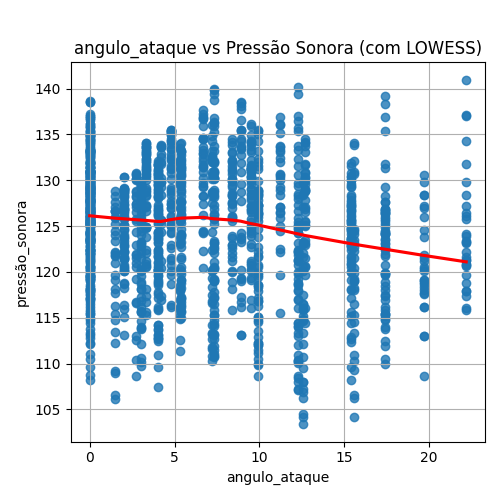
\includegraphics[width=\linewidth]{img/t1_disperssao_lowess_angulo_ataque}
	\caption{Ângulo (graus) vs Pressão Sonora (dB)}
	\label{fig:t1disperssaolowessanguloataque}
\end{subfigure} 
\begin{subfigure}{0.5\textwidth}
	\centering
	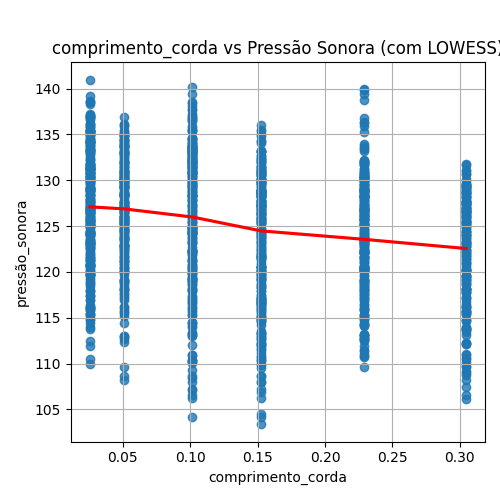
\includegraphics[width=\linewidth]{img/t1_disperssao_lowess_comprimento_corda}
	\caption{Comprimento (m) vs Pressão Sonora (dB)}
	\label{fig:t1disperssaolowesscomprimentocorda}
\end{subfigure}
\caption{Ângulo de Ataque, Comprimento da Corda vs Pressão Sonora}
\end{figure}

Na \fig{fig:t1disperssaolowessvelocidadefluxo} a curva é ligeiramente ascendente, mas bem suave. Mostra uma influência fraca, mas crescente da velocidade no aumento da pressão sonora. Reforça a correlação positiva fraca vista anteriormente.

\begin{figure}[H]
	\begin{subfigure}{0.5\textwidth}
	\centering
	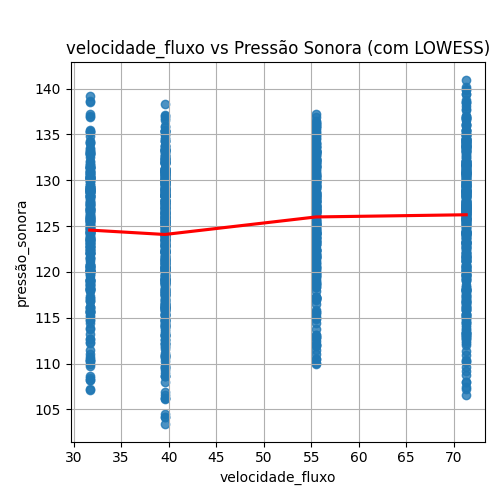
\includegraphics[width=\linewidth]{img/t1_disperssao_lowess_velocidade_fluxo}
	\caption{Velocidade (m/s) vs Pressão Sonora (dB)}
	\label{fig:t1disperssaolowessvelocidadefluxo}
		\end{subfigure} 
\begin{subfigure}{0.5\textwidth}
	\centering
	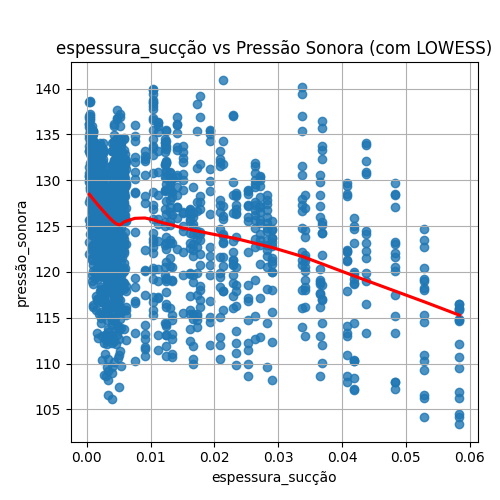
\includegraphics[width=\linewidth]{img/t1_disperssao_lowess_espessura_sucção}
	\caption{Espessura  (m) vs Pressão Sonora (dB)}
	\label{fig:t1disperssaolowessespessurasuccao}
\end{subfigure}
\caption{Velocidade de Fluxo e Espessura de Sucção vs Pressão Sonora}
\end{figure}

Na \fig{fig:t1disperssaolowessespessurasuccao} a curva é descendente, com alguma variação suave. Mostra uma relação inversa não linear: maior espessura tende a reduzir o ruído. Pode ser uma variável significativa no modelo.

Ao analisar as Figuras \ref{fig:t1disperssaolowessanguloataque} até \ref{fig:t1disperssaolowessespessurasuccao} inferimos que as variáveis \texttt{frequência} e \texttt{espessura de sucção} apresentam relações não lineares moderadamente fortes com a saída e devem ser valorizadas no modelo. As outras variáveis têm relações fracas, mas ainda assim podem ser relevantes em interações não lineares, que a rede neural pode capturar bem.

%\subsection{Histogramas}

%TODO: histograma aqui
	
	\subsection{Correla\c{c}\~ao dos Dados}
	
	Em estatística, a correlação é qualquer relação estatística, causal ou não, entre duas variáveis aleatórias. Segundo \citeauthor{silva:2023}, a correlação entre duas variáveis denota o grau em que as variáveis estão linearmente relacionadas. Ou seja, é uma medida de quanto as variáveis se relacionam em termos de força e direção.
	
	\subsubsection{Matriz de Correlação de Pearson}
	
	A matriz de correlação de Pearson é uma tabela que mostra o coeficiente de correlação de Pearson entre pares de variáveis numéricas. Cada valor na matriz mede a intensidade e direção da relação linear entre duas variáveis.
	
	O \textbf{Coeficiente de Pearson (r)} é um valor entre $-1$ e $+1$, onde :
	\begin{itemize}
		\item $1 \rightarrow$ correlação linear positiva perfeita: quando uma variável aumenta, a outra também aumenta.
		\item $-1 \rightarrow$ correlação linear negativa perfeita: quando uma variável aumenta, a outra diminui.
		\item $0 \rightarrow$ sem correlação linear: não há tendência linear entre as variáveis.
	\end{itemize}
	
	Existe mais de um método diferente de medir a relação entre duas variáveis, mas o mais conhecido e utilizado é o coeficiente de correlação de Pearson que avalia a rela\c{c}\~ao linear entre variáveis da seguinte forma\cite{silva:2023}:
	\begin{equation}
		r = \frac{\sum (x_i - \bar{x})(y_i - \bar{y})}{\sqrt{\sum (x_i - \bar{x})^2 \sum (y_i - \bar{y})^2}}
	\end{equation}
onde $\bar{x}$, $\bar{y}$: médias das variáveis.

O numerador é a covariância entre $x$ e $y$. O denominador normaliza pela variabilidade (desvio padrão) de cada variável.

Quando temos várias variáveis $x_1, x_2, \ldots, x_n$, a matriz de correlação é uma matriz $n \times n$ onde a posição $(i, j)$ representa a correlação entre $x_i$ e $x_j$ e a diagonal é sempre 1 (uma variável é perfeitamente correlacionada com ela mesma).

A matriz de correlação de Person é confiável para entender como os dados se comportam e é extremamente útil para identificar relações fortes entre entradas e saída. Além disso, Pode revelar colinearidade entre entradas, o que pode causar problemas em alguns modelos.
\begin{figure}[h]
	\centering
	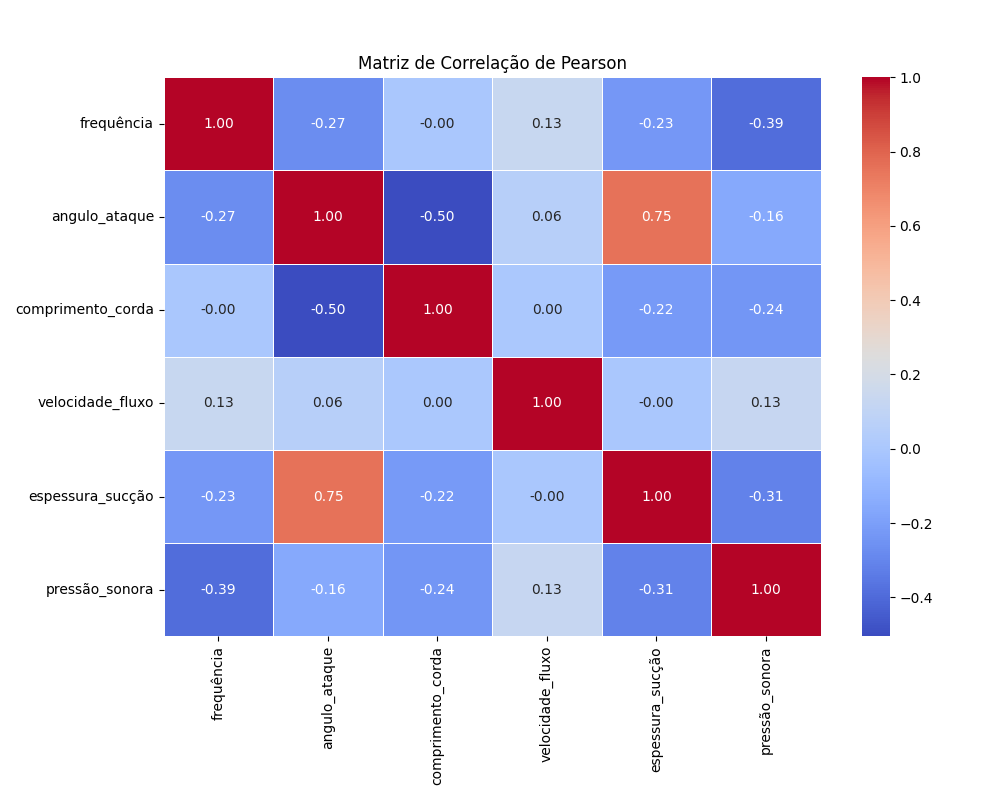
\includegraphics[width=0.7\linewidth]{img/t1_matriz_correlacao}
	\caption{Matriz de correlação de Person.}
	\label{fig:t1matrizcorrelacao}
\end{figure}

	Na Figura \ref{fig:t1matrizcorrelacao} matriz de correla\c{c}\~ao revelou que as variáveis frequência e espessura de suc\c{c}\~ao têm maior correla\c{c}\~ao com a press\~ao sonora. Além disso, inferimos as seguintes correlações com a variável alvo pressão sonora.
	 %Variável	Correlação com pressão\_sonora	Interpretação
	%Através da Figura \ref{fig:t1matrizcorrelacao}
	\texttt{Frequência}: correlação de $-0,39$, portanto avaliada como moderada e negativa. Isso significa que quanto maior a frequência, menor tende a ser a pressão sonora. Isso indica que frequência é relevante, com tendência inversa.
	 
	\texttt{Ângulo de ataque}: correlação de $-0,16$, ou seja, fraca e negativa. A influência do ângulo de ataque na pressão sonora é fraca, mas há uma leve tendência inversa.
	
	\texttt{Comprimento da corda}: correlação de $-0,24$, isto é, entre fraca a moderada negativa. Exite alguma influência da corda na redução da pressão sonora.
	
	\texttt{Velocidade de fluxo}: correlação $0,13$, logo avaliada como fraca e positiva. Têm pouca influência direta, mas há uma leve tendência de aumento da pressão sonora com velocidade.
	
	\texttt{Espessura de sucção}: correlação de $-0,31$, logo moderada e negativa. Mostra uma influência inversa: deslocamentos maiores tendem a reduzir a pressão sonora.
	
	Portanto as variáveis mais relevantes, com base na correlação linear, são: \texttt{Frequência} (correlação negativa moderada), a \texttt{Espessura de sucção} (correlação negativa moderada) e \texttt{Comprimento da corda} (correlação fraca a moderada negativa).
	
	
	\subsection{Outliers e Normaliza\c{c}\~ao}
	
	Outliers s\~ao valores extremos que podem distorcer o treinamento de modelos. Detectá-los ajuda a entender a confiabilidade dos dados.
	
	Verificá-los é importante porque podem distorcer o aprendizado da rede neural, fazendo com que o modelo foque demais nesses pontos raros. Além disso podem influenciar estatísticas como média e variância, prejudicando normalizações. Algumas redes neurais (especialmente com sigmoide ou tanh) são sensíveis a variações extremas, pois suas ativações saturam.
	
	\subsubsection*{Normalização}
	
	Normalizar os dados (trazer para uma mesma escala) é essencial para evitar que variáveis com grande escala (ex: frequência em Hz) dominem as de escala pequena (ex: comprimento em m). Além disso, acelera o treinamento, melhora a convergência do otimizador e deixa o espaço de entrada mais bem condicionado para modelos como redes neurais.
	
	Durante a análise dos dados foi constatado que há regi\~oes pouco cobertas nos dados, principalmente em valores extremos de frequência e espessura, o que pode comprometer a generaliza\c{c}\~ao do modelo. A normalização contribui para uma cobertura mais abrangente e confiável dos dados ao eliminar anomalias e otimizar a forma como os dados são tratados.


Na etapa de pré-processamento, um dos objetivos foi identificar possíveis outliers que pudessem afetar o desempenho do modelo. Para isso, utilizamos o escore Z (Z-score), que mede a distância de cada valor em relação à média da variável, em unidades de desvio padrão:

\begin{equation}
	z = \frac{x - \mu}{\sigma}
\end{equation}

Onde $x$ é o valor observado, $\mu$ é a média e $\sigma$ é o desvio padrão da variável. Valores de $|z| > 3$ são comumente considerados outliers. Essa escolha baseia-se em dois fundamentos:

\begin{itemize}
	\item \textbf{Distribuição Normal:} em uma distribuição aproximadamente normal, cerca de 99,7\% dos dados estão dentro de três desvios padrão da média. Logo, valores fora desse intervalo são estatisticamente raros.
	\item \textbf{Teorema de Chebyshev\cite{wiki:2025}:} independentemente da distribuição, ao menos 88,9\% dos dados devem estar dentro de $\pm 3\sigma$. Assim, $|z| > 3$ representa uma abordagem conservadora e robusta para identificação de valores extremos.
\end{itemize}

Portanto, o critério $|z| > 3$ é uma prática estatisticamente fundamentada para diagnóstico de outliers, sendo particularmente útil em bases de dados experimentais como esta. Na tabela \ref{tab:outliers_variables} realizamos a contagem de outliers por variáveis com base no Z-score $|z| > 3$.
\begin{table}[H]
	\centering
	\caption{Contagem de outliers por variável com base no Z-score}
	\label{tab:outliers_variables}
	\begin{tabular}{l c}
		\toprule
		\textbf{Variável} & \textbf{Outliers} \\
		\midrule
		Frequência                     & 44 \\
		Ângulo de ataque              & 0 \\
		Comprimento da corda          & 0 \\
		Velocidade do fluxo livre     & 0 \\
		Espessura de sucção           & 32 \\
		Pressão sonora                & 2 \\
		\bottomrule
	\end{tabular}
\end{table}
	
	\section{Treinamento do Multi-Layer Perceptron}
	
	Na Seção~\ref{sec:introducao}, apresentamos os fundamentos teóricos do perceptron multicamada (MLP), e na Seção~\ref{sec:impl_mlp}, desenvolvemos a dedução formal do algoritmo de retropropagação de erro aplicado à arquitetura da nossa rede, composta por 5 entradas, 10 neurônios na camada intermediária e 1 saída. Para a implementação e treinamento do modelo, utilizamos a biblioteca TensorFlow, amplamente consolidada no meio acadêmico e em aplicações de produção. A construção prática da MLP com TensorFlow foi detalhada na Seção~\ref{sec:mpl_tf}, e o código completo encontra-se disponível no Apêndice~\ref{appendix:A}.
	
	O modelo desenvolvido nesse trabalho possui as seguintes configura\c{c}\~oes:
	\begin{itemize}
		\item 1 camada intermediária com 10 neurônios;
		\item Função de ativa\c{c}\~ao sigmoide;
		\item Otimizador Adam com taxa de aprendizado com decaimento exponencial;
		\item Função de perda Erro Quadrático Médio (MSE);
		\item Mini-batch com 32 amostras;
		\item Treinamento realizado em 1000 épocas.
	\end{itemize}
	
	Após o treinamento as seguintes métricas foram utilizadas para avaliar o modelo:
	
	\paragraph{Erro Quadrático Médio (MSE)}: Definida na Equação (\ref{eq:mse}), o MSE calcula a média dos quadrados das diferenças entre os valores previstos e reais. Quanto menor o valor do MSE, melhor a qualidade do modelo, indicando menor erro entre as previsões e os valores observados.
	
	\paragraph{Erro Absoluto Médio (MAE)}: é uma métrica usada para medir a precisão de um modelo de regressão.
	
	\paragraph{Erro Absoluto Médio Relativo (RAE)}: é uma métrica que mede a média dos erros absolutos relativos entre os valores previstos e reais. Também é utilizado para avaliar a precisão de modelos preditivos, especialmente em situações onde é importante considerar a proporção do erro em relação ao valor real. 
	
	\paragraph{Coeficiente de Determinação (R\textsuperscript{2})}: é uma medida estatística que representa a qualidade do ajuste de um modelo de regressão. O valor do R\textsuperscript{2} está entre 0 e 1. Valor próximo de 1 indica um bom ajuste, enquanto próximo de 0 indica ajuste ruim.\cite{geeksforgeeks:2024}
	
	Além disso, foram gerados gráficos de resíduos e de valores reais vs preditos. Esses resultados mostram o desempenho do modelo e seu comportamento.
	
	Na Tabela \ref{tab:results_train} temos o resultado do treinamento para as seguintes métricas: MSE, MAE, R\textsuperscript{2} e RAE. Nela podemos observar que o MSE é baixo o que significa que temos um bom modelo. Isso é confirmado pelo MAE e RAE que estão próximos de zero. No caso do RAE valores baixos significa que a previsão do modelo é melhor que calcular a média. Para R\textsuperscript{2} próximo de 1 significa que modelo explica bem a variabilidade.
	\begin{table}[H]
		\centering
		\caption{Resultado do treinamento}
		\label{tab:results_train}
		\begin{tabular}{l c}
			\toprule
			\textbf{Métrica} & \textbf{Valor} \\
			\midrule
			MSE         & 0,1595 \\
			MAE         & 0,2929 \\
			RAE			& 0,3481\\
			R\textsuperscript{2}          & 0,8485 \\
			\bottomrule
		\end{tabular}
	\end{table}

\begin{figure}[h!]
	\centering
	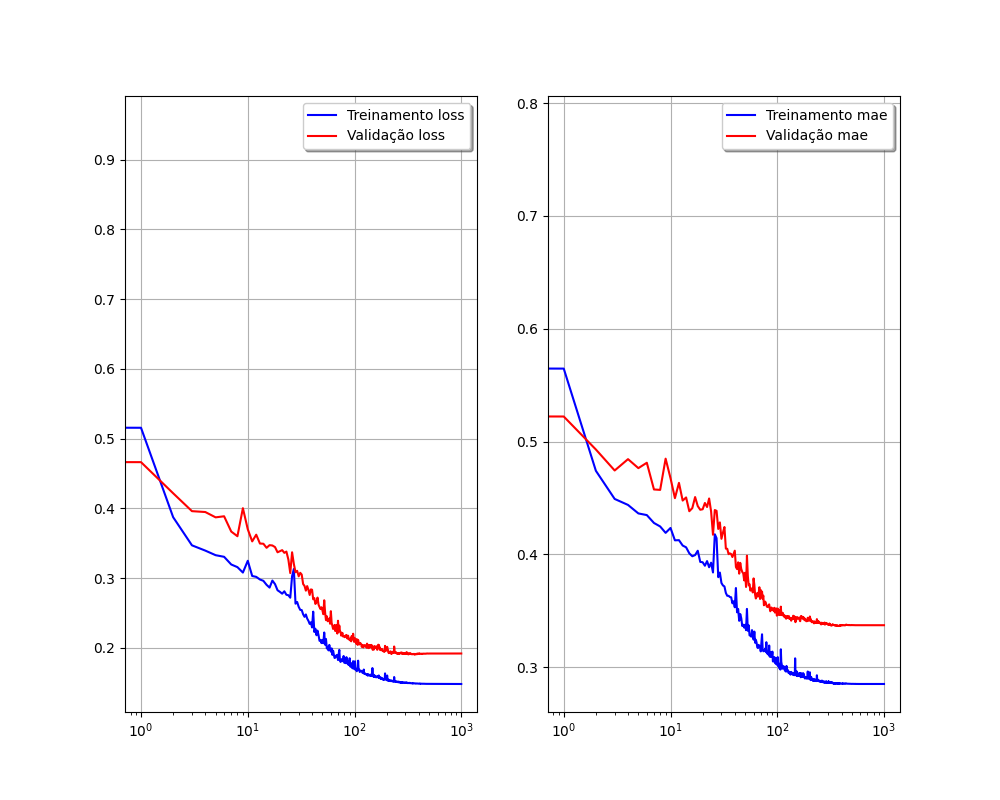
\includegraphics[width=0.7\linewidth]{img/t1_training_validation}
	\caption{Treino e validação.}
	\label{fig:t1trainingvalidation}
\end{figure}
	Na \fig{fig:t1trainingvalidation} temos dois gráficos o primeiro faz comparação entre a função de perda (MSE) e a validação cruzada. O segundo tem o mesmo objetivo, mas compara o MAE com a validação cruzada. A validação cruzada é útil para avaliar o desempenho do modelo e detecta a presença de \textit{overfitting}. 
	

Na \fig{fig:t1trainingvalidation} ambos os gráficos apresentaram uma curva decrescente ao longo do treinamento e não só isso, nas primeiras iterações o valor do erro no treinamento é maior, mas ao longo das iterações esse valor cai abaixo da validação cruzada. Esse comportamento já era esperado, pois a validação mede o desempenho em dados não vistos. Como a diferença entre as duas curvas é pequena o modelo está se ajustando melhor ao treino do que à validação.
	
%	Gráfico de resíduos:
%	
%	Distribuição aleatória em torno de 0 → ótimo.
%	Padrões, curvas, cones → o modelo está deixando passar padrões.
	
	Na Figura \ref{fig:t1residuos} temos o gráfico de resíduo que mostra a diferença entre os valores reais e os preditos pelo modelo. Ele é definido por $\text{resíduo} = (y_{real} - y_{predito})$. No eixo horizontal são representados os valores preditos e no eixo vertical são representados os resíduos. 
	\begin{figure}[h!]
		\centering
		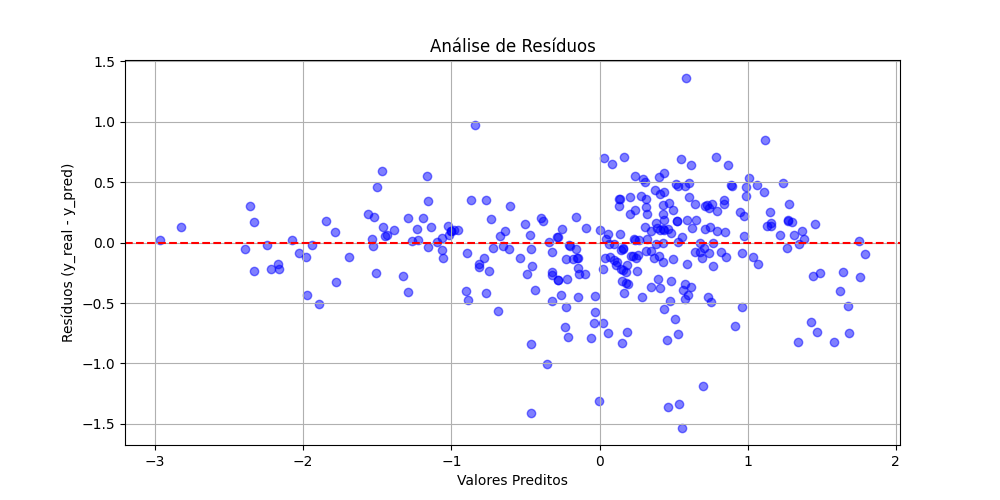
\includegraphics[width=0.7\linewidth]{img/t1_residuos}
		\caption{Resíduos $(y_{real} - y_{predito})$}
		\label{fig:t1residuos}
	\end{figure}

Os valores estão centrados em zero sem desvios aparente, isso significa que o modelo não apresenta vieses, ou seja, não tende a errar mais para cima ou para baixo. A maioria dos pontos estão dentro de uma amplitude entre $-1$ e $1$, isso significa que a maioria dos erros está dentro de 1 unidade da saída real, o que sugere boa precisão nas previsões.  
	
	
Na Figura \ref{fig:t1valoresreaispreditosleg} apresentamos um gráfico comparando os valores reais com os preditos. A linha tracejada é o caso ideal, ou seja, todos os valores coincidem. O objetivo é avaliar a dispersão dos valores ao redor do valor ideal. Como podemos observar a maioria dos pontos estão próximos da linha diagonal,ou seja, o modelo está fazendo boas previsões. Desvios grandes da linha indicam erros sistemáticos ou outliers. Os pontos não estão bem próximos dessa linha, isso implica que o modelo não tem boa precisão global.
	%Padrões ou distorções (curvas, faixas verticais) podem indicar problemas específicos, como erro em regiões extremas.
	\begin{figure}[h!]
		\centering
		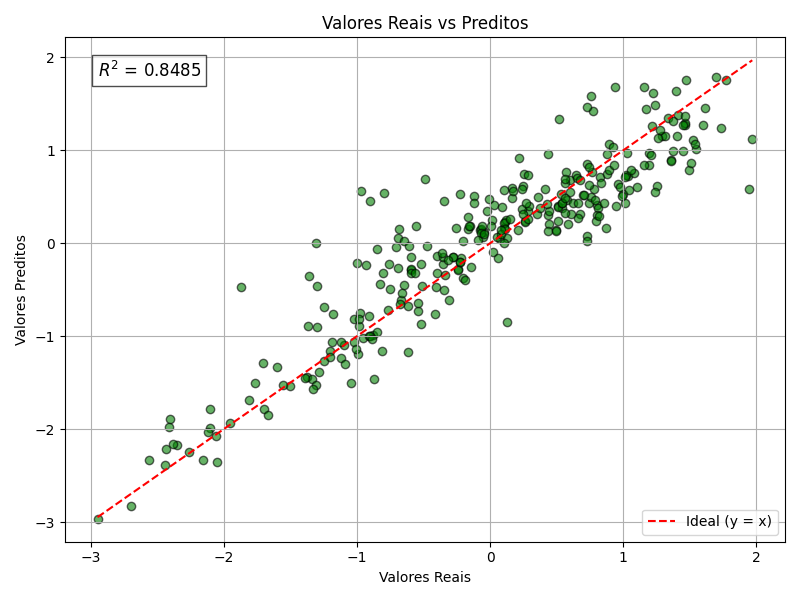
\includegraphics[width=0.7\linewidth]{img/t1_valores_reais_preditos_leg}
		\caption{Valores Reais vs Preditos.}
		\label{fig:t1valoresreaispreditosleg}
	\end{figure}
	
	\subsection{Experimentos}
	
	\paragraph{Experimento 1: Varia\c{c}\~ao do número de neurônios}
	
	O objetivo é verificar em que momento adicionar mais neurônios na camada intermediária deixa de melhorar o desempenho. Na Figura \ref{fig:t1_impacto_neuronio_performace} observou-se que após certo limite entre $10^{2}$ e $10^{3}$, o R\textsuperscript{2} se manteve estável.% Ao se aproximar de valores próximos de $10^{3}$ o coeficiente de determinação diminuiu.
	Após $10^{3}$ os valores de R\textsuperscript{2} começaram a oscilar, indicando risco de overfitting. Para evitar subajuste nos casos onde o número de neurônios é grande decidimos fixar um limiar (\textit{threshold}) ao invés do número de épocas. O limiar escolhido foi o erro absoluto médio menor que $0,1$, essa escolha seguiu o seguinte critério: Como o nível de pressão sonora varia entre aproximadamente $103 \text{ dB}$ e $141 \text{ dB}$, com desvio padrão de $6,9 \text{ dB}$, um erro médio absoluto de $0,1 \text{ dB}$ representa apenas $1,4\%$ da variabilidade típica. Isso garante que o modelo teve números de épocas o suficientes para convergir.
	\begin{figure}[h!]
		\centering
		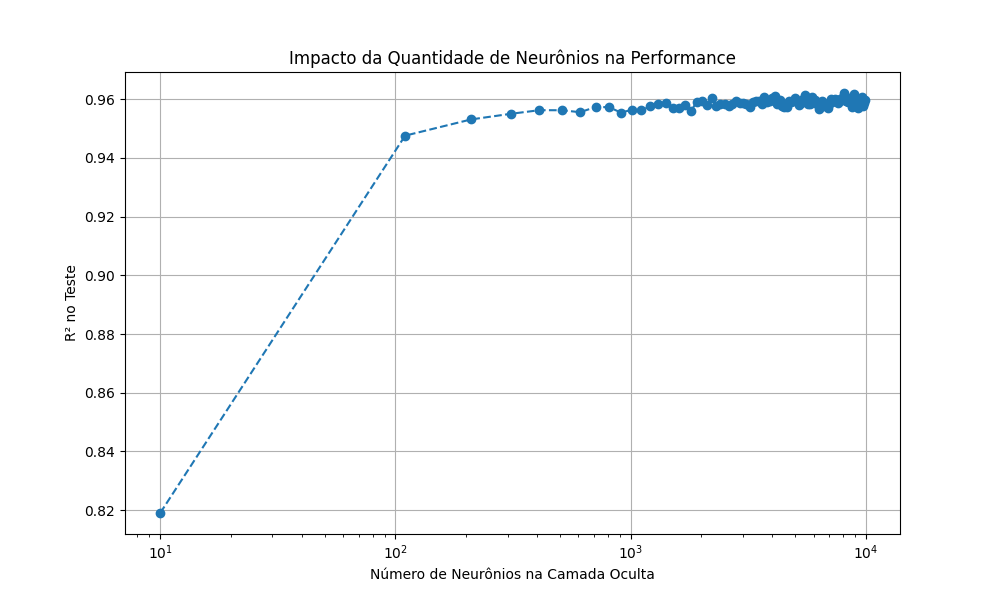
\includegraphics[width=0.7\linewidth]{img/t1_impacto_neuronio_performace}
		\caption{Treino e validação.}
		\label{fig:t1_impacto_neuronio_performace}
	\end{figure}
	
	A partir da Figura \ref{fig:t1_impacto_neuronio_performace} constatamos que a oscila no gráfico, quer dizer que aumentar a capacidade não melhora mais o modelo. Isso pode indicar que o problema tem baixa complexidade e poucos neurônios são suficientes. Nesse caso excesso de neurônios pode gerar \textit{overfitting} ou ineficiência computacional.
	
	\paragraph{Experimento 2: Comparar MLP e Regress\~ao Linear}
	
	Nesse experimento foi avaliado se usar uma rede neural realmente oferece vantagens em relação a um modelo clássico mais simples, como a regressão linear.
	
	A partir do mesmo conjunto de teste foi avaliado duas métricas que são MSE e o R\textsuperscript{2}. Se o R\textsuperscript{2} da MLP for significativamente maior, então vale a pena usar a rede neural. Caso contrário se a diferença for pequena, a simplicidade da regressão linear pode ser preferível.
	
	Os resultados comparando o desempenho entre MLP e a regressão linear está na \tab{tab:mlp_vs_reg_lin}:
	
	\begin{table}[H]
		\centering
		\caption{Comparação MLP vs Regressão Linear}
		\label{tab:mlp_vs_reg_lin}
		\begin{tabular}{l c c}
			\toprule
			& \textbf{MLP} & \textbf{Regressão Linear} \\
			\midrule
			MSE         & 0,1562 & 0,4650\\
			R\textsuperscript{2}    &  0,8516 & 0,5583   \\
			\bottomrule
		\end{tabular}
	\end{table}
	
	Os resultados mostraram que a MLP superou a regress\~ao linear em termos de R\textsuperscript{2}, validando seu uso para esse problema. A regressão linear é indicada para casos em que a relação linear é forte. Mas ao longo da nossa análise foi constatado que os dados possuem uma relação não linear e padrões complexos, caso ideal para utilizar uma rede neural.
	
	\paragraph{Experimento 3: Extrapola\c{c}\~ao com Dados Fora do Domínio}
	
%	Verificar como a rede neural se comporta ao fazer predições para dados que estão fora da faixa observada no treino, ou seja, situações onde não há garantia de cobertura do espaço de entrada. Esse tipo de análise é importante porque redes neurais são bons interpoladores, mas geralmente não extrapolam bem.
%	
%	A seguinte metodologia foi adotada nesse experimento:
%	
%	\begin{itemize}
%		\item Treinar a MLP com os dados normais.
%		\item Criar um conjunto de dados sintéticos fora da faixa dos dados de treino (ex: frequências muito altas, ângulos de ataque extremos).
%		\item Observar as predições e comparar com a tendência esperada.
%		\item Avaliar se a rede responde de forma consistente ou se gera valores absurdos.
%	\end{itemize} 
%	
%	Para um conjunto amostral de 10 pontos obtivemos o seguinte resultado:
%	\begin{verbatim}
%		Amostra 1: Pressão predita (extrapolada): -2.0962
%		Amostra 2: Pressão predita (extrapolada): -0.0904
%		Amostra 3: Pressão predita (extrapolada): -1.6585
%		Amostra 4: Pressão predita (extrapolada): -2.2081
%		Amostra 5: Pressão predita (extrapolada): -2.0871
%		Amostra 6: Pressão predita (extrapolada): -1.3351
%		Amostra 7: Pressão predita (extrapolada): 0.0839
%		Amostra 8: Pressão predita (extrapolada): -0.8269
%		Amostra 9: Pressão predita (extrapolada): -0.9036
%		Amostra 10: Pressão predita (extrapolada): -1.1660
%	\end{verbatim}
%	
%	Ao testarmos a MLP com entradas fora da faixa de treinamento as predi\c{c}\~oes se tornaram inconsistentes, confirmando que a MLP n\~ao é adequada para extrapola\c{c}\~oes, especialmente com ativa\c{c}\~oes sigmoides.
%	
%	Os valores retornados em sua maioria são negativos, isso mostra que a MLP não generaliza bem fora do intervalo dos dados. Extrapolação é sempre arriscada com redes neurais, especialmente com ativação sigmoide, que pode saturar.
%	
%	Portanto verificamos a varia\c{c}\~ao de hiper-parâmetros e sua influência no resultado final, e concluímos que mais complexidade n\~ao implica necessariamente em melhor desempenho.

Para avaliar a capacidade de generalização do modelo em situações que não foram observadas durante o treinamento, realizamos um experimento de extrapolação. Foram geradas 10 novas amostras de entrada, com valores de atributos propositalmente situados fora do intervalo dos dados originais. Nesse trabalho, foram utilizadas frequências entre $22.000$ e $30.000$ Hz, ângulos de ataque entre $15\degree$ e $25\degree$, e velocidades de fluxo superiores a $70$ m/s.

Essas amostras foram normalizadas utilizando a média e o desvio padrão do conjunto de treino original, e então submetidas à rede neural previamente treinada. As predições resultantes foram:

\begin{center}
	\small{
	\begin{tabular}{l|c c c c c c c c c l}
		\textbf{Amostra} & 1 & 2 & 3 & 4 & 5 & 6 & 7 & 8 & 9 & 10 \\ \hline
		\thead{Predição \\(normalizada)}  & 0,135 & 0,357 & 0,579 & 0,801 
		& 1,038 & 1,280 & 1,522 & 1,765 & 2,007 & 2,250 \\
	\end{tabular}
}
\end{center}

Aplicando a transformação inversa do Z-score com $\mu = 124{,}84$ e $\sigma = 6{,}74$, as predições foram convertidas para a escala original de decibéis, resultando em:

\begin{center}
	\small{
	\begin{tabular}{l|c c c c c c c c c l} 
		\textbf{Amostra} & 1 & 2 & 3 & 4 & 5 & 6 & 7 & 8 & 9 & 10 \\ \hline
		\thead{Predição \\(dB)}  & 125{,}76 & 127{,}25 & 128{,}74 & 130{,}23
		& 131{,}84 & 133{,}46 & 135{,}07 & 136{,}69 & 138{,}30 & 139{,}92  \\
	\end{tabular}
}
\end{center}

\begin{figure}[h!]
	\centering
	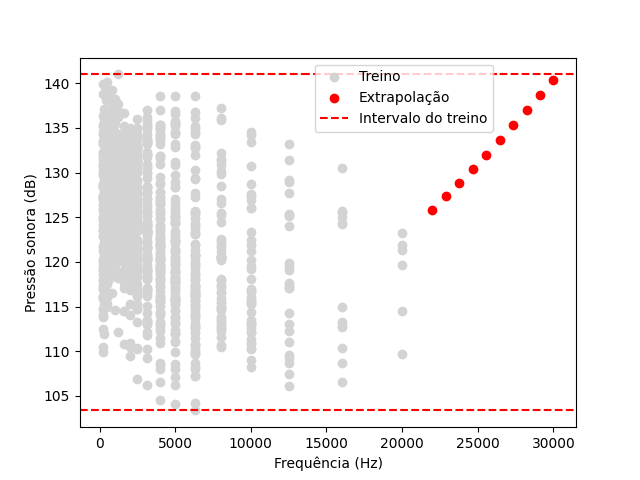
\includegraphics[width=0.7\linewidth]{img/extrapolacao.png}
	\caption{Treino e validação.}
	\label{fig:extrapolacao}
\end{figure}

Na Figura \ref{fig:extrapolacao} foi comparado o intervalo de saída dos dados de treino, entre $103{,}38$ dB e $140{,}99$ dB.  Observamos que todas as predições extrapoladas permanecem dentro dos limites observados. Além disso, os valores aumentam de forma contínua e suave, sugerindo que a rede neural captou uma tendência coerente mesmo fora do intervalo de treino.

Essa estabilidade na extrapolação indica que o modelo, apesar de treinado em um domínio limitado, é capaz de manter consistência nas predições para entradas razoavelmente extrapoladas. No entanto, é importante destacar que, quanto mais distante dos dados de treino forem os novos exemplos, maior será a incerteza das predições, especialmente em modelos com funções de ativação como a sigmoide, que podem saturar nas extremidades.
	
	\chapter{Conclus\~ao}
	
%	Este trabalho investigou a aplica\c{c}\~ao de uma rede neural MLP para prever a press\~ao sonora gerada por aerofólios. Através da análise crítica dos dados e experimentos, concluímos que:
%	
%	\begin{itemize}
%		\item O modelo foi capaz de capturar rela\c{c}\~oes complexas nos dados.
%		\item A MLP apresentou desempenho superior à regress\~ao linear.
%		\item A extrapola\c{c}\~ao dos dados mostrou limita\c{c}\~oes significativas.
%		\item As escolhas de arquitetura e parâmetros influenciam diretamente o desempenho.
%		\item O modelo se mostrou adequado dentro da faixa de treinamento, mas carece de robustez fora dela.
%	\end{itemize}

%\section*{Conclusão}

Este trabalho investigou a aplicação de redes neurais artificiais, em especial o modelo Multi-Layer Perceptron (MLP), para previsão da pressão sonora em aerofólios. O estudo envolveu desde a análise exploratória dos dados, até a implementação e avaliação de um modelo treinado com TensorFlow.

A análise estatística e gráfica revelou a importância da frequência e da espessura de sucção como variáveis de maior influência sobre a pressão sonora. O processo de normalização com Z-score e a remoção de outliers foram essenciais para melhorar a estabilidade e a capacidade de generalização do modelo.

A implementação do MLP com uma camada oculta e função sigmoide foi eficaz, atingindo bom desempenho em métricas como $R^2 =  0,8485$ e MSE baixo. A comparação com regressão linear confirmou a superioridade da rede neural para modelar padrões não lineares presentes nos dados.

Três experimentos complementares foram realizados: o primeiro demonstrou que há um ponto ótimo no número de neurônios, além do qual o desempenho se estabiliza ou piora; o segundo confirmou que a MLP supera modelos lineares em desempenho preditivo; e o terceiro evidenciou que, apesar das limitações naturais de extrapolação, a rede neural produziu predições coerentes e dentro da faixa física plausível para dados fora do domínio de treino. As predições aumentaram suavemente com as entradas e mantiveram-se dentro do intervalo real observado no conjunto de treino, reforçando a estabilidade do modelo.

Concluímos que a MLP é adequada para tarefas de regressão dentro de domínios bem representados no conjunto de treino. No entanto, sua capacidade de extrapolação é limitada, sendo essencial garantir a boa cobertura do espaço de entrada. A escolha cuidadosa da arquitetura, regularização e pré-processamento foram determinantes para o sucesso da modelagem.




%%%%%%%%%%%%%%%%%%%%%%%%%%%%%%%%%%%%%%%%%%%%%%%%%%%%%%%%%%%%%%%%%%%
%                  Referências Bibliográficas                     % 
%%%%%%%%%%%%%%%%%%%%%%%%%%%%%%%%%%%%%%%%%%%%%%%%%%%%%%%%%%%%%%%%%%%
\thispagestyle{empty}
\addcontentsline{toc}{chapter}{Referências Bibliográficas}
%
%\thispagestyle{myheadings}
\bibliography{bibtex}
\newpage
%%%%%%%%%%%%%%%%%%%%%%%%%%%%%%%%%%%%%%%%%%%%%%%%%%%%%%%%
%                         Apêndice                     % 
%%%%%%%%%%%%%%%%%%%%%%%%%%%%%%%%%%%%%%%%%%%%%%%%%%%%%%%%
\appendix

\chapter{Códigos Python para Regressão Logística}
\label{appendix:A}
\thispagestyle{empty}

\begin{lstlisting}[caption={Analise dos dados}, label={lst:analise_dados}]
import numpy as np
import pandas as pd
import matplotlib.pyplot as plt
from ucimlrepo import fetch_ucirepo 
import seaborn as sns
from scipy import stats

airfoil_self_noise = pd.read_table('./airfoil+self+noise/airfoil_self_noise.dat',
	names=["frequência","angulo_ataque","comprimento_corda","velocidade_fluxo",
	"espessura_sucção","pressão_sonora"])
X = airfoil_self_noise.iloc[:,0:5]
y = airfoil_self_noise.iloc[:,5:6]

# Gerar scatter plot com curva LOWESS para cada entrada
for coluna in airfoil_self_noise.columns[:-1]:  # Exclui a variável alvo
g=sns.lmplot(x=coluna,y='pressão_sonora',
data=airfoil_self_noise,lowess=True,line_kws={'color': 'red'})

g.ax.grid(True, axis='both')
sns.despine(fig=None, ax=None, top=False, right=False, left=False, bottom=False, offset=None, trim=False)
plt.title(f'{coluna} vs Pressão Sonora (com LOWESS)')
plt.xlabel(coluna)
plt.ylabel('pressão_sonora')
plt.tight_layout(rect=[0, 0, 1, 0.95])
plt.savefig(f'img/t1_disperssao_lowess_{coluna}.png',format='png')
plt.show()

# Calcular matriz de correlação
corr = airfoil_self_noise.corr()

# Visualizar com heatmap
plt.figure(figsize=(10, 8))
sns.heatmap(corr, annot=True, cmap='coolwarm', fmt=".2f", linewidths=0.5)
plt.title('Matriz de Correlação de Pearson')
plt.tight_layout(rect=[0, 0, 1, 0.95])
plt.savefig('img/t1_matriz_correlacao.png',format='png')
plt.show()

# 1. Detectar Outliers usando Z-score
z_scores = np.abs(stats.zscore(airfoil_self_noise))           # calcula z-score absoluto
outliers = z_scores > 3                        # define outliers como z > 3
outliers_por_variavel = pd.Series(np.sum(outliers, axis=0), index=airfoil_self_noise.columns)

#print("Quantidade de outliers por variável:")
outliers_por_variavel

# Configurar estilo dos gráficos
sns.set(style="whitegrid", font_scale=1.5)

# Criar boxplots para cada variável
fig, axes = plt.subplots(2, 3, figsize=(18, 10))  # cria um grid 2x3
axes = axes.flatten()  # achata para iterar facilmente

for idx, coluna in enumerate(airfoil_self_noise.columns):
sns.boxplot(data=airfoil_self_noise, x=coluna, ax=axes[idx], color='skyblue')
axes[idx].set_title(f'Boxplot de {coluna}')
axes[idx].set_xlabel("")  # remove o nome do eixo X para estética

plt.tight_layout()
plt.savefig('img/t1_boxplot.png',format='png')
plt.show()
\end{lstlisting}

\begin{lstlisting}[caption={Multi-Layer Perceptron}, label={lst:mpl_impl_all}]
import tensorflow as tf
from tensorflow.keras.models import Sequential
from tensorflow.keras.layers import Dense
from tensorflow.keras.optimizers.schedules import ExponentialDecay
from tensorflow.keras.optimizers import Adam
from sklearn.model_selection import train_test_split
import pandas as pd
from sklearn.metrics import r2_score

# 1. Carregar os dados normalizados
airfoil_self_noise = pd.read_table('./airfoil+self+noise/airfoil_self_noise.dat',
names=["frequência","angulo_ataque","comprimento_corda","velocidade_fluxo",
"espessura_sucção","pressão_sonora"])
df_normalizado = (airfoil_self_noise - airfoil_self_noise.mean()) / airfoil_self_noise.std()

X = df_normalizado.drop(columns=['pressão_sonora']).values
y = df_normalizado['pressão_sonora'].values

# 2. Dividir em treino e teste
X_train, X_test, y_train, y_test = train_test_split(X, y, test_size=0.2, random_state=42)

# 3. Definir taxa de aprendizado com decaimento exponencial
initial_lr = 0.01
lr_schedule = ExponentialDecay(initial_learning_rate=initial_lr,
decay_steps=100,decay_rate=0.96,staircase=True
)

# 4. Construir o modelo
model = Sequential([
Dense(100, activation='sigmoid', kernel_regularizer=regularizers.l2(0.001)
 input_shape=(X.shape[1],)), Dense(1, activation='linear')  # saída contínua
])

# 5. Compilar o modelo
model.compile(optimizer=Adam(learning_rate=lr_schedule),
loss='mse',metrics=['mae'])

# 6. Treinar o modelo
history = model.fit(X_train, y_train,epochs=2000,
batch_size=32,validation_split=0.2,verbose=1
)

# 7. Avaliar no conjunto de teste
test_loss, test_mae = model.evaluate(X_test, y_test)
print(f"Erro quadrático médio no teste: {test_loss:.4f}")
print(f"Erro absoluto médio no teste: {test_mae:.4f}")

#Vamos ver como foi o treino?
fig, ax = plt.subplots(1,2, figsize=(10,8))
ax[0].semilogx(history.history['loss'], color='b', label="Treinamento loss")
ax[0].semilogx(history.history['val_loss'], color='r', label="Validação loss")
legend = ax[0].legend(loc='best', shadow=True)

ax[1].semilogx(history.history['mae'], color='b', label="Treinamento mae")
ax[1].semilogx(history.history['val_mae'], color='r',label="Validação mae")
legend = ax[1].legend(loc='best', shadow=True)
plt.grid(True)
plt.savefig('img/t1_training_validation.png',format='png')

# 1. Predições do modelo
y_pred = model.predict(X_test).flatten()

# 2. Coeficiente de determinação (R^2)
r2 = r2_score(y_test, y_pred)
print(f"Coeficiente de determinação R^2: {r2:.4f}")

# 3. Erro Absoluto Médio Relativo (RAE)
rae = np.sum(np.abs(y_test - y_pred)) / np.sum(np.abs(y_test - np.mean(y_test)))
print(f"Erro Absoluto Médio Relativo (RAE): {rae:.4f}")

# 4. Análise gráfica de resíduos
residuos = y_test - y_pred

plt.figure(figsize=(10, 5))
plt.scatter(y_pred, residuos, alpha=0.5, color='blue')
plt.axhline(0, color='red', linestyle='--')
plt.xlabel('Valores Preditos')
plt.ylabel('Resíduos (y_real - y_pred)')
plt.title('Análise de Resíduos')
plt.grid(True)
plt.savefig('img/t1_residuos.png',format='png')
plt.show()

y_pred = model.predict(X_test).flatten()
r2 = r2_score(y_test, y_pred)

# Gráfico: valores reais vs preditos
plt.figure(figsize=(8, 6))
plt.scatter(y_test, y_pred, alpha=0.6, color='green', edgecolors='k')
plt.plot([y_test.min(), y_test.max()], [y_test.min(), y_test.max()], 'r--', label='Ideal (y = x)')

# Adiciona R^2 no gráfico
plt.text(x=min(y_test), y=max(y_pred), s=f"$R^2$ = {r2:.4f}", fontsize=12, color='black', bbox=dict(facecolor='white', alpha=0.7))

plt.xlabel('Valores Reais')
plt.ylabel('Valores Preditos')
plt.title('Valores Reais vs Preditos')
plt.legend()
plt.grid(True)
plt.tight_layout()
plt.savefig('img/t1_valores_reais_preditos_leg.png',format='png')
plt.show()

# Experimentos

# Lista para armazenar resultados
resultados = []
neuronios_testados = []

# Loop para testar diferentes quantidades de neurônios
for neuronios in range(10, 10000, 100):
	# Aprendizado com decaimento exponencial
	lr_schedule = ExponentialDecay(initial_learning_rate=0.01,
	decay_steps=100,decay_rate=0.96,staircase=True
	)
	
	# Modelo MLP
	model = Sequential([
	Dense(neuronios, activation='sigmoid', input_shape=(X.shape[1],)),
	Dense(1, activation='linear')
	])
	model.compile(optimizer=Adam(learning_rate=lr_schedule), loss='mse')
	model.fit(X_train, y_train, epochs=200, batch_size=32, verbose=0)
	
	# Avaliação
	y_pred = model.predict(X_test).flatten()
	r2 = r2_score(y_test, y_pred)
	resultados.append(r2)
	neuronios_testados.append(neuronios)

# Plotar os resultados
plt.figure(figsize=(10, 6))
plt.semilogx(neuronios_testados, resultados, marker='o', linestyle='--')
plt.xlabel("Número de Neurônios na Camada Oculta")
plt.ylabel(f"$R^2$ no Teste")
plt.title("Impacto da Quantidade de Neurônios na Performance")
plt.grid(True)
plt.savefig('img/t1_impacto_neuronio_performace.png',format='png')
plt.show()
\end{lstlisting}
	
\end{document}
